\documentclass{gmcm2026}
\graphicspath{{./}}
\begin{document}
\pagestyle{empty}
\renewcommand{\thefigure}{4.\arabic{figure}}
\setlength{\textfloatsep}{8pt plus 2pt minus 2pt}
\setlength{\abovecaptionskip}{4pt}
% 实际插入宽度 152mm（正文宽 165mm 的 92%）：图高 1054/724*152 = 221.3mm
% + 两行图注约 9.5mm + 浮动间距约 3.2mm ≈ 234mm ≤ 正文高 248.5mm，单页容纳
\begin{figure}[!htbp]
\centering
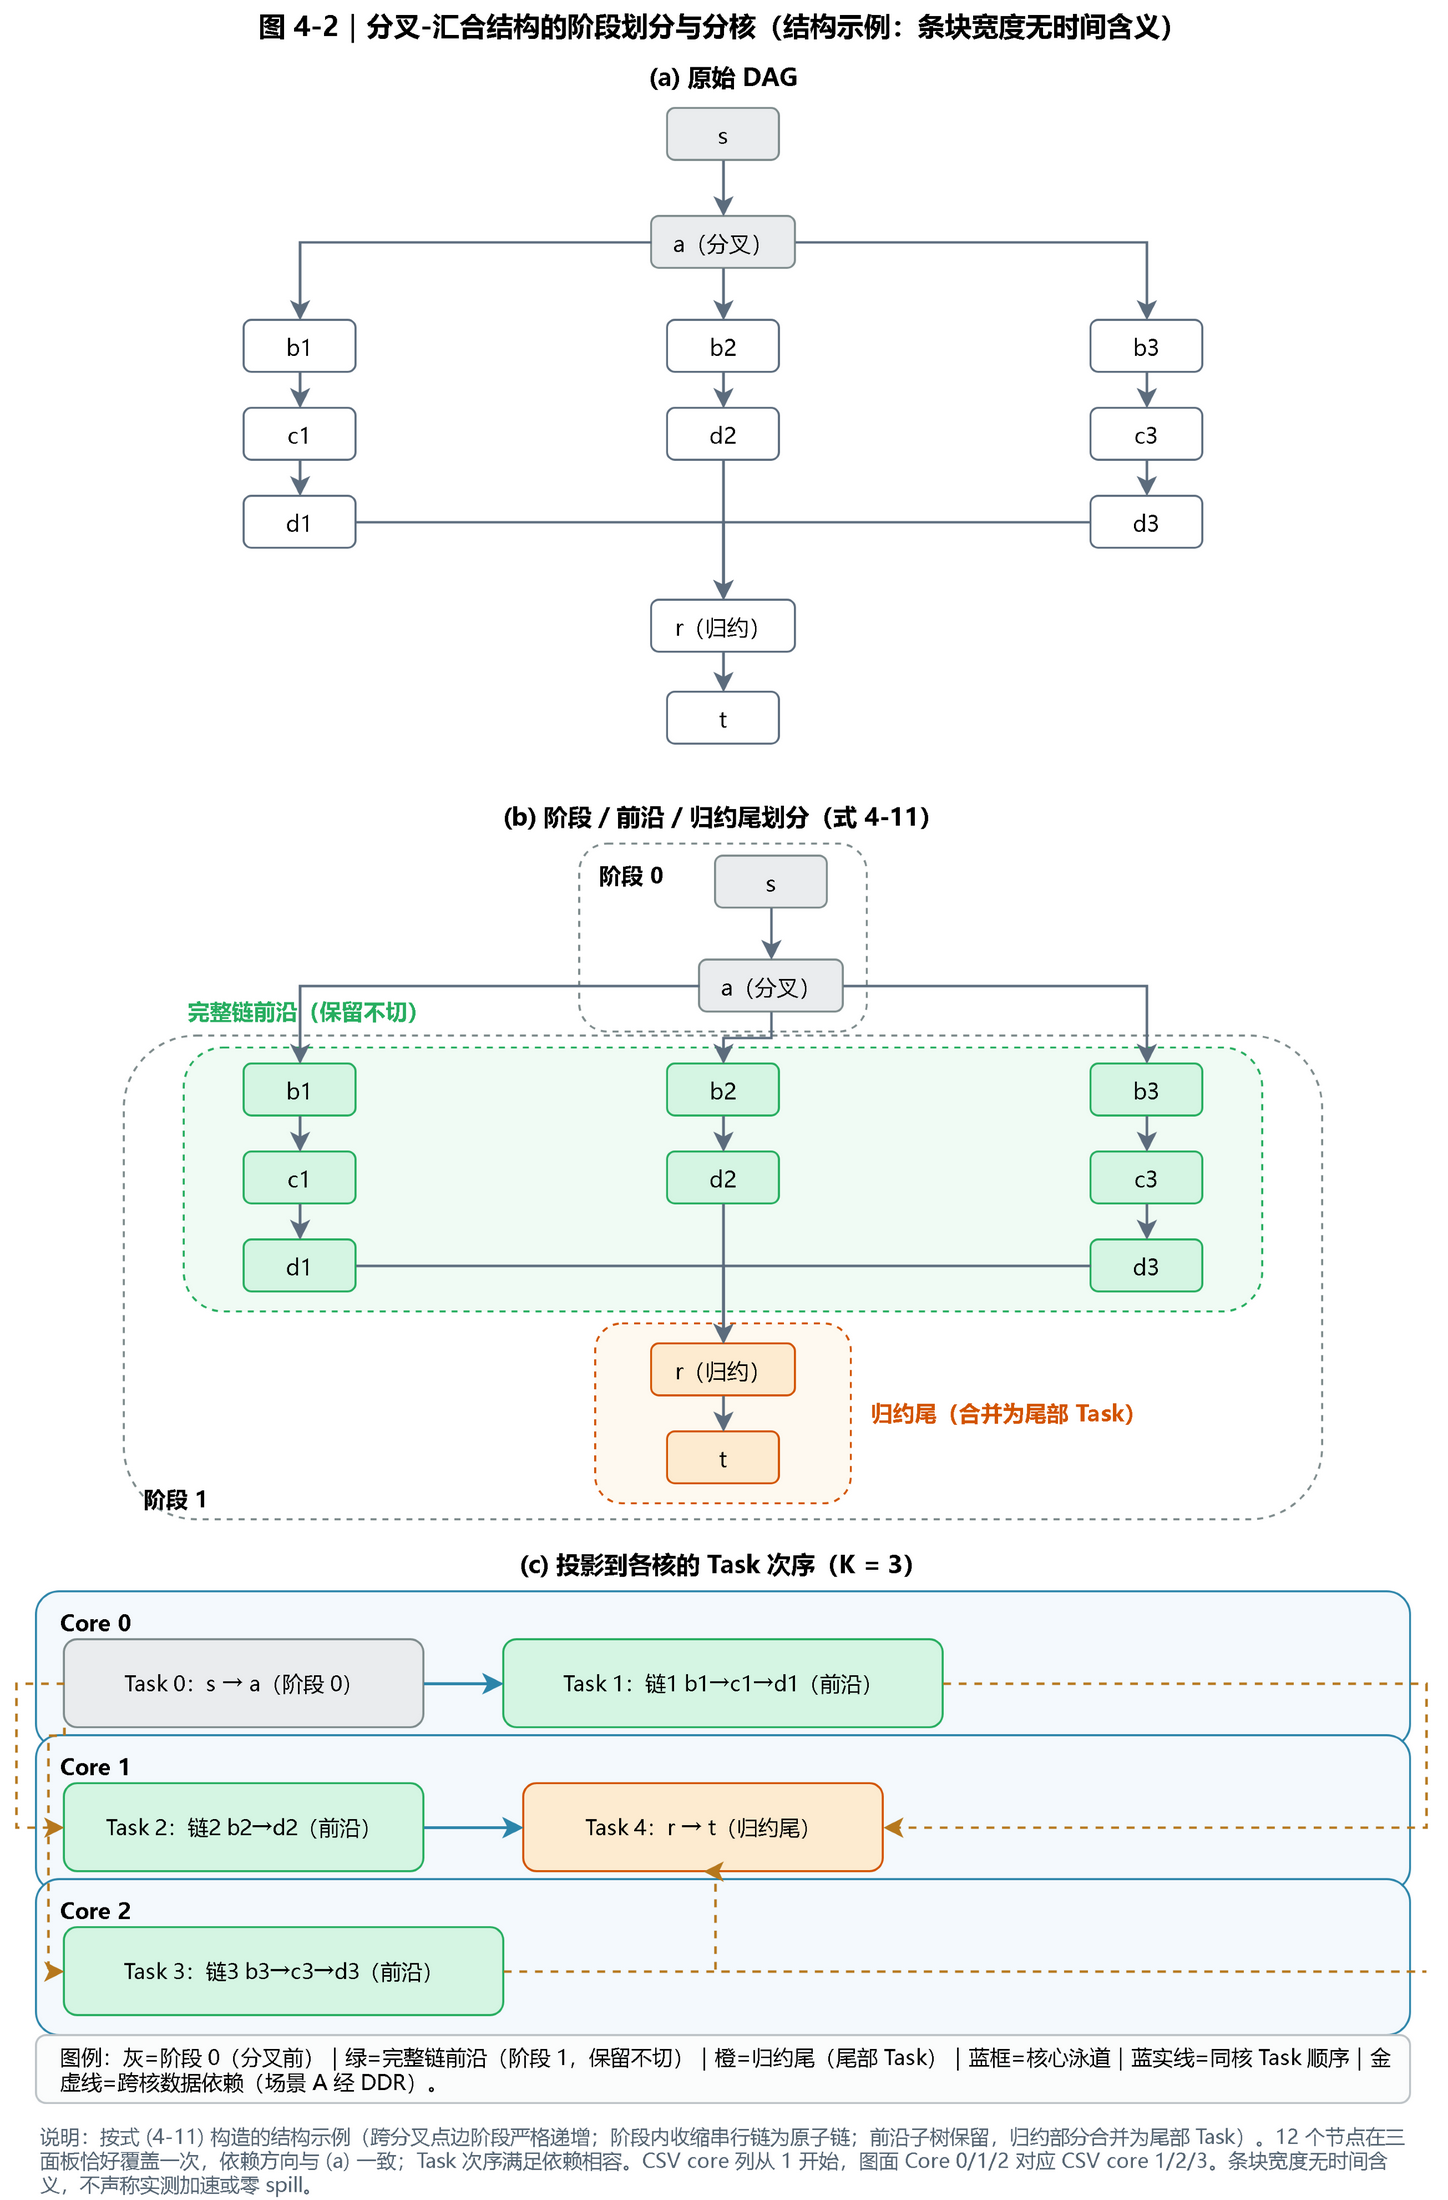
\includegraphics[width=152mm]{fig4-2-fork-join-partition.png}
\caption{分叉-汇合结构的阶段划分与分核：(a)~原始 DAG；(b)~式~(4-11) 阶段划分
（完整链前沿保留不切、归约尾合并）；(c)~$K{=}3$ 核 Task 次序（跨核依赖经 DDR）。
结构示例，条块宽度无时间含义，不声称实测加速或零 spill。}
\end{figure}
\end{document}
